\documentclass[twoside]{book}

% Packages required by doxygen
\usepackage{fixltx2e}
\usepackage{calc}
\usepackage{doxygen}
\usepackage[export]{adjustbox} % also loads graphicx
\usepackage{graphicx}
\usepackage[utf8]{inputenc}
\usepackage{makeidx}
\usepackage{multicol}
\usepackage{multirow}
\PassOptionsToPackage{warn}{textcomp}
\usepackage{textcomp}
\usepackage[nointegrals]{wasysym}
\usepackage[table]{xcolor}

% Font selection
\usepackage[T1]{fontenc}
\usepackage[scaled=.90]{helvet}
\usepackage{courier}
\usepackage{amssymb}
\usepackage{sectsty}
\renewcommand{\familydefault}{\sfdefault}
\allsectionsfont{%
  \fontseries{bc}\selectfont%
  \color{darkgray}%
}
\renewcommand{\DoxyLabelFont}{%
  \fontseries{bc}\selectfont%
  \color{darkgray}%
}
\newcommand{\+}{\discretionary{\mbox{\scriptsize$\hookleftarrow$}}{}{}}

% Page & text layout
\usepackage{geometry}
\geometry{%
  a4paper,%
  top=2.5cm,%
  bottom=2.5cm,%
  left=2.5cm,%
  right=2.5cm%
}
\tolerance=750
\hfuzz=15pt
\hbadness=750
\setlength{\emergencystretch}{15pt}
\setlength{\parindent}{0cm}
\setlength{\parskip}{3ex plus 2ex minus 2ex}
\makeatletter
\renewcommand{\paragraph}{%
  \@startsection{paragraph}{4}{0ex}{-1.0ex}{1.0ex}{%
    \normalfont\normalsize\bfseries\SS@parafont%
  }%
}
\renewcommand{\subparagraph}{%
  \@startsection{subparagraph}{5}{0ex}{-1.0ex}{1.0ex}{%
    \normalfont\normalsize\bfseries\SS@subparafont%
  }%
}
\makeatother

% Headers & footers
\usepackage{fancyhdr}
\pagestyle{fancyplain}
\fancyhead[LE]{\fancyplain{}{\bfseries\thepage}}
\fancyhead[CE]{\fancyplain{}{}}
\fancyhead[RE]{\fancyplain{}{\bfseries\leftmark}}
\fancyhead[LO]{\fancyplain{}{\bfseries\rightmark}}
\fancyhead[CO]{\fancyplain{}{}}
\fancyhead[RO]{\fancyplain{}{\bfseries\thepage}}
\fancyfoot[LE]{\fancyplain{}{}}
\fancyfoot[CE]{\fancyplain{}{}}
\fancyfoot[RE]{\fancyplain{}{\bfseries\scriptsize Generated by Doxygen }}
\fancyfoot[LO]{\fancyplain{}{\bfseries\scriptsize Generated by Doxygen }}
\fancyfoot[CO]{\fancyplain{}{}}
\fancyfoot[RO]{\fancyplain{}{}}
\renewcommand{\footrulewidth}{0.4pt}
\renewcommand{\chaptermark}[1]{%
  \markboth{#1}{}%
}
\renewcommand{\sectionmark}[1]{%
  \markright{\thesection\ #1}%
}

% Indices & bibliography
\usepackage{natbib}
\usepackage[titles]{tocloft}
\setcounter{tocdepth}{3}
\setcounter{secnumdepth}{5}
\makeindex

% Hyperlinks (required, but should be loaded last)
\usepackage{ifpdf}
\ifpdf
  \usepackage[pdftex,pagebackref=true]{hyperref}
\else
  \usepackage[ps2pdf,pagebackref=true]{hyperref}
\fi
\hypersetup{%
  colorlinks=true,%
  linkcolor=blue,%
  citecolor=blue,%
  unicode%
}

% Custom commands
\newcommand{\clearemptydoublepage}{%
  \newpage{\pagestyle{empty}\cleardoublepage}%
}

\usepackage{caption}
\captionsetup{labelsep=space,justification=centering,font={bf},singlelinecheck=off,skip=4pt,position=top}

%===== C O N T E N T S =====

\begin{document}

% Titlepage & ToC
\hypersetup{pageanchor=false,
             bookmarksnumbered=true,
             pdfencoding=unicode
            }
\pagenumbering{alph}
\begin{titlepage}
\vspace*{7cm}
\begin{center}%
{\Large Cliente Consumidor }\\
\vspace*{1cm}
{\large Generated by Doxygen 1.8.14}\\
\end{center}
\end{titlepage}
\clearemptydoublepage
\pagenumbering{roman}
\tableofcontents
\clearemptydoublepage
\pagenumbering{arabic}
\hypersetup{pageanchor=true}

%--- Begin generated contents ---
\chapter{Namespace Index}
\section{Lista de Namespaces}
Esta é a lista de todos os Namespaces com suas respectivas descrições\+:\begin{DoxyCompactList}
\item\contentsline{section}{\mbox{\hyperlink{namespace_ui}{Ui}} }{\pageref{namespace_ui}}{}
\end{DoxyCompactList}

\chapter{Hierarchical Index}
\section{Hierarquia de Classes}
Esta lista de hierarquias está parcialmente ordenada (ordem alfabética)\+:\begin{DoxyCompactList}
\item Q\+Main\+Window\begin{DoxyCompactList}
\item \contentsline{section}{Main\+Window}{\pageref{class_main_window}}{}
\end{DoxyCompactList}
\end{DoxyCompactList}

\chapter{Class Index}
\section{Class List}
Here are the classes, structs, unions and interfaces with brief descriptions\+:\begin{DoxyCompactList}
\item\contentsline{section}{\mbox{\hyperlink{class_main_window}{Main\+Window}} }{\pageref{class_main_window}}{}
\item\contentsline{section}{\mbox{\hyperlink{class_plotter}{Plotter}} }{\pageref{class_plotter}}{}
\end{DoxyCompactList}

\chapter{File Index}
\section{File List}
Here is a list of all files with brief descriptions\+:\begin{DoxyCompactList}
\item\contentsline{section}{C\+:/\+Users/mateu/\+Documents/\+Cliente\+\_\+\+Consumidor/\mbox{\hyperlink{main_8cpp}{main.\+cpp}} }{\pageref{main_8cpp}}{}
\item\contentsline{section}{C\+:/\+Users/mateu/\+Documents/\+Cliente\+\_\+\+Consumidor/\mbox{\hyperlink{mainwindow_8cpp}{mainwindow.\+cpp}} }{\pageref{mainwindow_8cpp}}{}
\item\contentsline{section}{C\+:/\+Users/mateu/\+Documents/\+Cliente\+\_\+\+Consumidor/\mbox{\hyperlink{mainwindow_8h}{mainwindow.\+h}} }{\pageref{mainwindow_8h}}{}
\item\contentsline{section}{C\+:/\+Users/mateu/\+Documents/\+Cliente\+\_\+\+Consumidor/\mbox{\hyperlink{plotter_8cpp}{plotter.\+cpp}} }{\pageref{plotter_8cpp}}{}
\item\contentsline{section}{C\+:/\+Users/mateu/\+Documents/\+Cliente\+\_\+\+Consumidor/\mbox{\hyperlink{plotter_8h}{plotter.\+h}} }{\pageref{plotter_8h}}{}
\end{DoxyCompactList}

\chapter{Namespace Documentation}
\hypertarget{namespace_ui}{}\section{Ui Namespace Reference}
\label{namespace_ui}\index{Ui@{Ui}}

\chapter{Class Documentation}
\hypertarget{class_main_window}{}\section{Main\+Window Class Reference}
\label{class_main_window}\index{Main\+Window@{Main\+Window}}


{\ttfamily \#include $<$mainwindow.\+h$>$}

Inheritance diagram for Main\+Window\+:\begin{figure}[H]
\begin{center}
\leavevmode
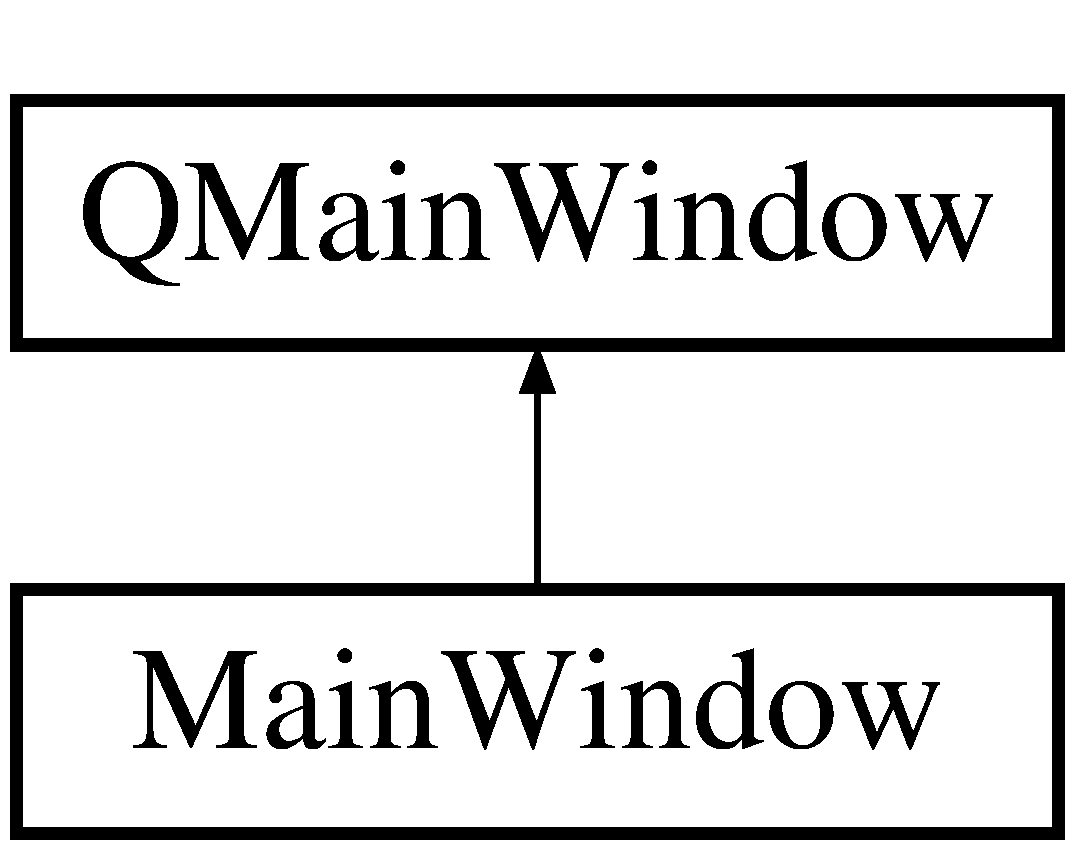
\includegraphics[height=2.000000cm]{class_main_window}
\end{center}
\end{figure}
\subsection*{Public Slots}
\begin{DoxyCompactItemize}
\item 
void \mbox{\hyperlink{class_main_window_a26b6030035e196b64333906db8302cdd}{tcp\+Connect}} (void)
\begin{DoxyCompactList}\small\item\em Realiza conexão com o server. \end{DoxyCompactList}\item 
void \mbox{\hyperlink{class_main_window_a3389bbbe4222f115a7609037a1a63bd5}{tcp\+Disconnect}} (void)
\begin{DoxyCompactList}\small\item\em Desconecta do server. \end{DoxyCompactList}\item 
void \mbox{\hyperlink{class_main_window_ac6d3a5fa8ef8ede69436b9e9a6ee80c1}{get\+Data}} (void)
\begin{DoxyCompactList}\small\item\em Captura dados do servidor de acordo com o tempo determinado pelo user. \end{DoxyCompactList}\item 
void \mbox{\hyperlink{class_main_window_a2e3dceeb08f18cc1d07e42b79fe7a0c1}{stop\+Data}} (void)
\begin{DoxyCompactList}\small\item\em Para a captura de dados. \end{DoxyCompactList}\item 
void \mbox{\hyperlink{class_main_window_a6d5ab019a97676b4edfe7d4b6a541455}{update\+Ip}} (void)
\begin{DoxyCompactList}\small\item\em Mostra uma lista dos clientes conectados. \end{DoxyCompactList}\item 
void \mbox{\hyperlink{class_main_window_a9d08a694a5f9c532225754381b8011ea}{timer\+Event}} (Q\+Timer\+Event $\ast$e)
\begin{DoxyCompactList}\small\item\em Função que determina o tempo da captura de dados definido pelo user. \end{DoxyCompactList}\end{DoxyCompactItemize}
\subsection*{Public Member Functions}
\begin{DoxyCompactItemize}
\item 
\mbox{\hyperlink{class_main_window_a8b244be8b7b7db1b08de2a2acb9409db}{Main\+Window}} (Q\+Widget $\ast$parent=0)
\item 
\mbox{\hyperlink{class_main_window_ae98d00a93bc118200eeef9f9bba1dba7}{$\sim$\+Main\+Window}} ()
\end{DoxyCompactItemize}


\subsection{Constructor \& Destructor Documentation}
\mbox{\Hypertarget{class_main_window_a8b244be8b7b7db1b08de2a2acb9409db}\label{class_main_window_a8b244be8b7b7db1b08de2a2acb9409db}} 
\index{Main\+Window@{Main\+Window}!Main\+Window@{Main\+Window}}
\index{Main\+Window@{Main\+Window}!Main\+Window@{Main\+Window}}
\subsubsection{\texorpdfstring{Main\+Window()}{MainWindow()}}
{\footnotesize\ttfamily Main\+Window\+::\+Main\+Window (\begin{DoxyParamCaption}\item[{Q\+Widget $\ast$}]{parent = {\ttfamily 0} }\end{DoxyParamCaption})\hspace{0.3cm}{\ttfamily [explicit]}}


\begin{DoxyCode}
13                                       :
14     QMainWindow(parent),
15     ui(\textcolor{keyword}{new} Ui::MainWindow)
16 \{
17     ui->setupUi(\textcolor{keyword}{this});
18     socket = \textcolor{keyword}{new} QTcpSocket(\textcolor{keyword}{this});
19     idTimer = 0;
20 
21     connect(ui->pushButtonGet,
22             SIGNAL(clicked(\textcolor{keywordtype}{bool})),
23             \textcolor{keyword}{this},
24             SLOT(\mbox{\hyperlink{class_main_window_ac6d3a5fa8ef8ede69436b9e9a6ee80c1}{getData}}()));
25     connect(ui->pushButton\_Stop,
26             SIGNAL(clicked(\textcolor{keywordtype}{bool})),
27             \textcolor{keyword}{this},
28             SLOT(\mbox{\hyperlink{class_main_window_a2e3dceeb08f18cc1d07e42b79fe7a0c1}{stopData}}()));
29     connect(ui->pushButton\_Connect,
30             SIGNAL(clicked(\textcolor{keywordtype}{bool})),
31             \textcolor{keyword}{this},
32             SLOT(\mbox{\hyperlink{class_main_window_a26b6030035e196b64333906db8302cdd}{tcpConnect}}()));
33     connect(ui->pushButton\_Disconnect,
34             SIGNAL(clicked(\textcolor{keywordtype}{bool})),
35             \textcolor{keyword}{this},
36             SLOT(\mbox{\hyperlink{class_main_window_a3389bbbe4222f115a7609037a1a63bd5}{tcpDisconnect}}()));
37     connect(ui->pushButton\_Update,
38             SIGNAL(clicked(\textcolor{keywordtype}{bool})),
39             \textcolor{keyword}{this},
40             SLOT(\mbox{\hyperlink{class_main_window_a6d5ab019a97676b4edfe7d4b6a541455}{updateIp}}()));
41 \}
\end{DoxyCode}
\mbox{\Hypertarget{class_main_window_ae98d00a93bc118200eeef9f9bba1dba7}\label{class_main_window_ae98d00a93bc118200eeef9f9bba1dba7}} 
\index{Main\+Window@{Main\+Window}!````~Main\+Window@{$\sim$\+Main\+Window}}
\index{````~Main\+Window@{$\sim$\+Main\+Window}!Main\+Window@{Main\+Window}}
\subsubsection{\texorpdfstring{$\sim$\+Main\+Window()}{~MainWindow()}}
{\footnotesize\ttfamily Main\+Window\+::$\sim$\+Main\+Window (\begin{DoxyParamCaption}{ }\end{DoxyParamCaption})}


\begin{DoxyCode}
170 \{
171     \textcolor{keyword}{delete} socket;
172     \textcolor{keyword}{delete} ui;
173 \}
\end{DoxyCode}


\subsection{Member Function Documentation}
\mbox{\Hypertarget{class_main_window_ac6d3a5fa8ef8ede69436b9e9a6ee80c1}\label{class_main_window_ac6d3a5fa8ef8ede69436b9e9a6ee80c1}} 
\index{Main\+Window@{Main\+Window}!get\+Data@{get\+Data}}
\index{get\+Data@{get\+Data}!Main\+Window@{Main\+Window}}
\subsubsection{\texorpdfstring{get\+Data}{getData}}
{\footnotesize\ttfamily void Main\+Window\+::get\+Data (\begin{DoxyParamCaption}\item[{void}]{ }\end{DoxyParamCaption})\hspace{0.3cm}{\ttfamily [slot]}}



Captura dados do servidor de acordo com o tempo determinado pelo user. 


\begin{DoxyCode}
58                         \{
59     \textcolor{keywordflow}{if}(idTimer)\{
60         killTimer(idTimer);
61     \}
62     idTimer = startTimer(ui->horizontalSlider\_Time->value()*1000);
63 
64 \}
\end{DoxyCode}
\mbox{\Hypertarget{class_main_window_a2e3dceeb08f18cc1d07e42b79fe7a0c1}\label{class_main_window_a2e3dceeb08f18cc1d07e42b79fe7a0c1}} 
\index{Main\+Window@{Main\+Window}!stop\+Data@{stop\+Data}}
\index{stop\+Data@{stop\+Data}!Main\+Window@{Main\+Window}}
\subsubsection{\texorpdfstring{stop\+Data}{stopData}}
{\footnotesize\ttfamily void Main\+Window\+::stop\+Data (\begin{DoxyParamCaption}\item[{void}]{ }\end{DoxyParamCaption})\hspace{0.3cm}{\ttfamily [slot]}}



Para a captura de dados. 


\begin{DoxyCode}
143                              \{
144     \textcolor{keywordflow}{if}(idTimer)\{
145         killTimer(idTimer);
146     \}
147 \}
\end{DoxyCode}
\mbox{\Hypertarget{class_main_window_a26b6030035e196b64333906db8302cdd}\label{class_main_window_a26b6030035e196b64333906db8302cdd}} 
\index{Main\+Window@{Main\+Window}!tcp\+Connect@{tcp\+Connect}}
\index{tcp\+Connect@{tcp\+Connect}!Main\+Window@{Main\+Window}}
\subsubsection{\texorpdfstring{tcp\+Connect}{tcpConnect}}
{\footnotesize\ttfamily void Main\+Window\+::tcp\+Connect (\begin{DoxyParamCaption}\item[{void}]{ }\end{DoxyParamCaption})\hspace{0.3cm}{\ttfamily [slot]}}



Realiza conexão com o server. 


\begin{DoxyCode}
43                            \{
44     socket->connectToHost(ui->lineEdit\_Host->text(),1234);
45     \textcolor{keywordflow}{if}(socket->waitForConnected())\{
46         qDebug() << \textcolor{stringliteral}{"Connected"};
47     \}
48     \textcolor{keywordflow}{else}\{
49         qDebug() << \textcolor{stringliteral}{"Disconnected"};
50     \}
51 \}
\end{DoxyCode}
\mbox{\Hypertarget{class_main_window_a3389bbbe4222f115a7609037a1a63bd5}\label{class_main_window_a3389bbbe4222f115a7609037a1a63bd5}} 
\index{Main\+Window@{Main\+Window}!tcp\+Disconnect@{tcp\+Disconnect}}
\index{tcp\+Disconnect@{tcp\+Disconnect}!Main\+Window@{Main\+Window}}
\subsubsection{\texorpdfstring{tcp\+Disconnect}{tcpDisconnect}}
{\footnotesize\ttfamily void Main\+Window\+::tcp\+Disconnect (\begin{DoxyParamCaption}\item[{void}]{ }\end{DoxyParamCaption})\hspace{0.3cm}{\ttfamily [slot]}}



Desconecta do server. 


\begin{DoxyCode}
53                               \{
54     socket->disconnectFromHost();
55 \}
\end{DoxyCode}
\mbox{\Hypertarget{class_main_window_a9d08a694a5f9c532225754381b8011ea}\label{class_main_window_a9d08a694a5f9c532225754381b8011ea}} 
\index{Main\+Window@{Main\+Window}!timer\+Event@{timer\+Event}}
\index{timer\+Event@{timer\+Event}!Main\+Window@{Main\+Window}}
\subsubsection{\texorpdfstring{timer\+Event}{timerEvent}}
{\footnotesize\ttfamily void Main\+Window\+::timer\+Event (\begin{DoxyParamCaption}\item[{Q\+Timer\+Event $\ast$}]{e }\end{DoxyParamCaption})\hspace{0.3cm}{\ttfamily [slot]}}



Função que determina o tempo da captura de dados definido pelo user. 


\begin{DoxyCode}
66                                          \{
67     QString str;
68     QStringList list;
69     qint64 thetime, num;
70     \textcolor{keywordtype}{double} max\_x, min\_x, min\_y, max\_y;
71     std::vector<double> time;
72     std::vector<double> data;
73     std::vector<double> temposnorm;
74     std::vector<double> dadosnorm;
75 
76     qDebug() << \textcolor{stringliteral}{"to get data..."};
77     \textcolor{keywordflow}{if}(socket->state() == QAbstractSocket::ConnectedState)\{
78         \textcolor{keywordflow}{if}(socket->isOpen())\{
79             qDebug() << \textcolor{stringliteral}{"reading..."};
80             str = \textcolor{stringliteral}{"get "} + ui->listWidget\_ListaDeClients->currentItem()->text() + \textcolor{stringliteral}{" 30\(\backslash\)r\(\backslash\)n"};
81             socket->write(str.toStdString().c\_str());
82             socket->waitForBytesWritten();
83             socket->waitForReadyRead();
84             qDebug() << socket->bytesAvailable();
85             time.clear();
86             data.clear();
87             \textcolor{keywordflow}{while}(socket->bytesAvailable())\{
88                 str = socket->readLine().replace(\textcolor{stringliteral}{"\(\backslash\)n"},\textcolor{stringliteral}{""}).replace(\textcolor{stringliteral}{"\(\backslash\)r"},\textcolor{stringliteral}{""});
89                 list = str.split(\textcolor{stringliteral}{" "});
90 
91                 \textcolor{keywordflow}{if}(list.size() == 2)\{
92                     \textcolor{keywordtype}{bool} ok;
93                     str = list.at(0);
94                     thetime = str.toLongLong(&ok);
95                     time.push\_back(thetime);
96 
97                     str = list.at(1);
98                     num = str.toLongLong(&ok);
99                     data.push\_back(num);
100                     qDebug() << thetime << \textcolor{stringliteral}{": "} << str;
101                 \}
102             \}
103         \}
104     \}
105 
106     qDebug()<<data.size()<<time.size();
107     \textcolor{comment}{//achando valores maximos e minimos}
108     max\_x = time[0], min\_x = time[0];
109     min\_y = data[0], max\_y = data[0];
110 
111     \textcolor{keywordflow}{for}(\textcolor{keywordtype}{int} i = 1 ; i < 30; i++)\{
112         \textcolor{keywordflow}{if}(time[i] < min\_x)\{
113             min\_x = time[i];
114         \}
115         \textcolor{keywordflow}{else} \textcolor{keywordflow}{if}(time[i] > max\_x)\{
116             max\_x = time[i];
117         \}
118         \textcolor{keywordflow}{if}(data[i] < min\_y)\{
119             min\_y = data[i];
120         \}
121         \textcolor{keywordflow}{else} \textcolor{keywordflow}{if}(data[i] > max\_y)\{
122             max\_y = data[i];
123         \}
124     \}
125 
126     qDebug()<<max\_x-min\_x;
127 
128 
129     qDebug()<<max\_y<<min\_y;
130 
131 
132     \textcolor{comment}{//normalizando dados}
133     temposnorm.clear();
134     dadosnorm.clear();
135     \textcolor{keywordflow}{for}(\textcolor{keywordtype}{int} i = 0; i<30; i++)\{
136         temposnorm.push\_back((time[i] - min\_x)/(max\_x - min\_x));
137         dadosnorm.push\_back((data[i] - min\_y)/(max\_y - min\_y));
138     \}
139     qDebug()<<\textcolor{stringliteral}{"passou"};
140     ui->widget\_Plotter->loadData(temposnorm,dadosnorm);
141 \}
\end{DoxyCode}
\mbox{\Hypertarget{class_main_window_a6d5ab019a97676b4edfe7d4b6a541455}\label{class_main_window_a6d5ab019a97676b4edfe7d4b6a541455}} 
\index{Main\+Window@{Main\+Window}!update\+Ip@{update\+Ip}}
\index{update\+Ip@{update\+Ip}!Main\+Window@{Main\+Window}}
\subsubsection{\texorpdfstring{update\+Ip}{updateIp}}
{\footnotesize\ttfamily void Main\+Window\+::update\+Ip (\begin{DoxyParamCaption}\item[{void}]{ }\end{DoxyParamCaption})\hspace{0.3cm}{\ttfamily [slot]}}



Mostra uma lista dos clientes conectados. 


\begin{DoxyCode}
149                              \{
150     QString str;
151 
152     ui->listWidget\_ListaDeClients->clear();
153     \textcolor{keywordflow}{if}(socket->state() == QAbstractSocket::ConnectedState)\{
154         socket->write(\textcolor{stringliteral}{"list\(\backslash\)r\(\backslash\)n"});
155         socket->waitForBytesWritten();
156         socket->waitForReadyRead();
157         \textcolor{keywordflow}{while}(socket->bytesAvailable())\{
158             str = socket->readLine().replace(\textcolor{stringliteral}{"\(\backslash\)n"},\textcolor{stringliteral}{""}).replace(\textcolor{stringliteral}{"\(\backslash\)r"},\textcolor{stringliteral}{""});
159             ui->listWidget\_ListaDeClients->addItem(str);
160         \}
161     \}
162     \textcolor{keywordflow}{else}\{
163         ui->listWidget\_ListaDeClients->addItem(\textcolor{stringliteral}{"Lista vazia"});
164     \}
165 
166 \}
\end{DoxyCode}


The documentation for this class was generated from the following files\+:\begin{DoxyCompactItemize}
\item 
C\+:/\+Users/mateu/\+Documents/\+Cliente\+\_\+\+Consumidor/\mbox{\hyperlink{mainwindow_8h}{mainwindow.\+h}}\item 
C\+:/\+Users/mateu/\+Documents/\+Cliente\+\_\+\+Consumidor/\mbox{\hyperlink{mainwindow_8cpp}{mainwindow.\+cpp}}\end{DoxyCompactItemize}

\hypertarget{class_plotter}{}\section{Plotter Class Reference}
\label{class_plotter}\index{Plotter@{Plotter}}


{\ttfamily \#include $<$plotter.\+h$>$}

Inheritance diagram for Plotter\+:\begin{figure}[H]
\begin{center}
\leavevmode
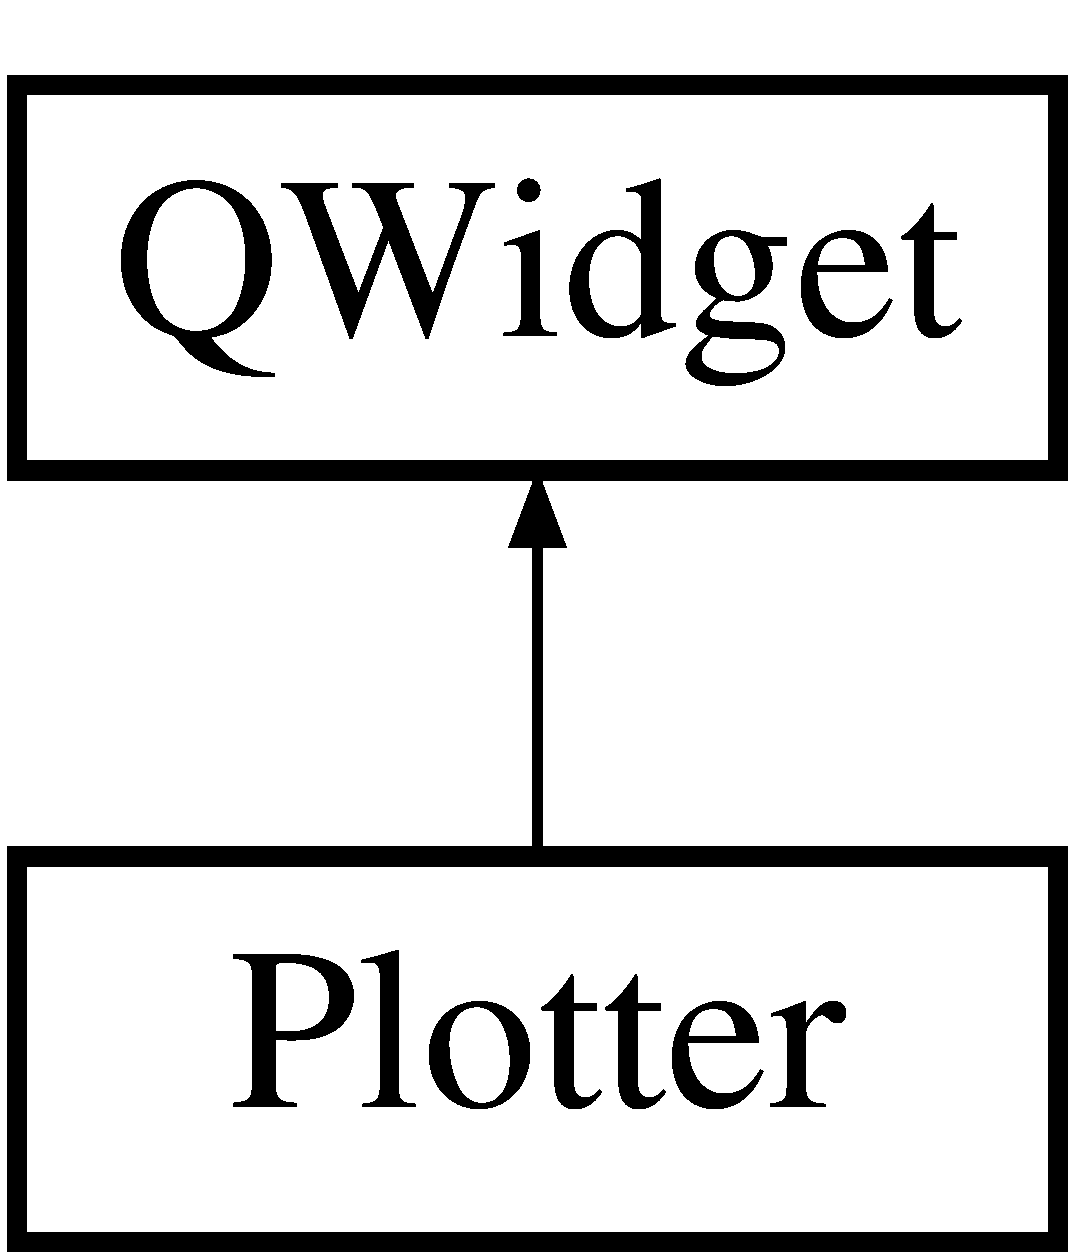
\includegraphics[height=2.000000cm]{class_plotter}
\end{center}
\end{figure}
\subsection*{Public Member Functions}
\begin{DoxyCompactItemize}
\item 
\mbox{\hyperlink{class_plotter_a367b6890c36910a27ec710ac3693e64b}{Plotter}} (Q\+Widget $\ast$parent=0)
\begin{DoxyCompactList}\small\item\em Construtor do \mbox{\hyperlink{class_plotter}{Plotter}}. \end{DoxyCompactList}\item 
void \mbox{\hyperlink{class_plotter_ac4341569909943e37e1ff756587e6e12}{paint\+Event}} (Q\+Paint\+Event $\ast$e)
\begin{DoxyCompactList}\small\item\em Desenha retas através de pares de pontos. \end{DoxyCompactList}\item 
void \mbox{\hyperlink{class_plotter_ae73b5093b98bbbebd6abdb4e7e7807ed}{load\+Data}} (std\+::vector$<$ double $>$, std\+::vector$<$ double $>$)
\begin{DoxyCompactList}\small\item\em Função que carrega os dados e os prepara para mostrar no gráfico. \end{DoxyCompactList}\end{DoxyCompactItemize}


\subsection{Constructor \& Destructor Documentation}
\mbox{\Hypertarget{class_plotter_a367b6890c36910a27ec710ac3693e64b}\label{class_plotter_a367b6890c36910a27ec710ac3693e64b}} 
\index{Plotter@{Plotter}!Plotter@{Plotter}}
\index{Plotter@{Plotter}!Plotter@{Plotter}}
\subsubsection{\texorpdfstring{Plotter()}{Plotter()}}
{\footnotesize\ttfamily Plotter\+::\+Plotter (\begin{DoxyParamCaption}\item[{Q\+Widget $\ast$}]{parent = {\ttfamily 0} }\end{DoxyParamCaption})\hspace{0.3cm}{\ttfamily [explicit]}}



Construtor do \mbox{\hyperlink{class_plotter}{Plotter}}. 


\begin{DoxyCode}
11                                 :
12     QWidget(parent)\{
13     \textcolor{keywordflow}{for}(\textcolor{keywordtype}{int} i=0; i<30; i++)\{
14         tempos.push\_back(i);
15         dados.push\_back(i);
16     \}
17 \}
\end{DoxyCode}


\subsection{Member Function Documentation}
\mbox{\Hypertarget{class_plotter_ae73b5093b98bbbebd6abdb4e7e7807ed}\label{class_plotter_ae73b5093b98bbbebd6abdb4e7e7807ed}} 
\index{Plotter@{Plotter}!load\+Data@{load\+Data}}
\index{load\+Data@{load\+Data}!Plotter@{Plotter}}
\subsubsection{\texorpdfstring{load\+Data()}{loadData()}}
{\footnotesize\ttfamily void Plotter\+::load\+Data (\begin{DoxyParamCaption}\item[{std\+::vector$<$ double $>$}]{,  }\item[{std\+::vector$<$ double $>$}]{ }\end{DoxyParamCaption})}



Função que carrega os dados e os prepara para mostrar no gráfico. 


\begin{DoxyCode}
60                                                         \{
61     tempos=t;
62     dados=d;
63     repaint();
64 \}
\end{DoxyCode}
\mbox{\Hypertarget{class_plotter_ac4341569909943e37e1ff756587e6e12}\label{class_plotter_ac4341569909943e37e1ff756587e6e12}} 
\index{Plotter@{Plotter}!paint\+Event@{paint\+Event}}
\index{paint\+Event@{paint\+Event}!Plotter@{Plotter}}
\subsubsection{\texorpdfstring{paint\+Event()}{paintEvent()}}
{\footnotesize\ttfamily void Plotter\+::paint\+Event (\begin{DoxyParamCaption}\item[{Q\+Paint\+Event $\ast$}]{e }\end{DoxyParamCaption})}



Desenha retas através de pares de pontos. 


\begin{DoxyCode}
20 \{
21     QPainter painter(\textcolor{keyword}{this});
22     QBrush brush;
23     QPen pen;
24     \textcolor{keywordtype}{double} x1, x2, y1, y2;
25 
26     painter.setRenderHint(QPainter::Antialiasing);
27 
28     brush.setColor(QColor(255,255,200));
29     brush.setStyle(Qt::SolidPattern);
30 
31 \textcolor{comment}{//    pen.setColor(QColor(255,0,0));}
32 \textcolor{comment}{//    pen.setWidth(3);}
33 
34     painter.setBrush(brush);
35     painter.setPen(pen);
36 
37     \textcolor{comment}{// desenha o fundo do plotter}
38     painter.drawRect(0,0,width(), height());
39 
40     pen.setColor(QColor(0,0,255));
41     pen.setWidth(2);
42     pen.setStyle(Qt::SolidLine);
43     painter.setPen(pen);
44 
45     \textcolor{comment}{//plotando graficos}
46 
47     x1 = tempos[0]*width();
48     y1 = dados[0]*(height()-dados[0]);
49 
50     \textcolor{keywordflow}{for}(\textcolor{keywordtype}{int} i=1; i<30; i++)\{
51         x2=tempos[i]*width();
52         y2=dados[i]*(height()-dados[i]);
53         painter.drawLine(x1,y1,x2,y2);
54         x1 = x2;
55         y1 = y2;
56     \}
57 
58 \}
\end{DoxyCode}


The documentation for this class was generated from the following files\+:\begin{DoxyCompactItemize}
\item 
C\+:/\+Users/mateu/\+Documents/\+Cliente\+\_\+\+Consumidor/\mbox{\hyperlink{plotter_8h}{plotter.\+h}}\item 
C\+:/\+Users/mateu/\+Documents/\+Cliente\+\_\+\+Consumidor/\mbox{\hyperlink{plotter_8cpp}{plotter.\+cpp}}\end{DoxyCompactItemize}

\chapter{File Documentation}
\hypertarget{main_8cpp}{}\section{Referência do Arquivo C\+:/\+Users/mateu/\+Documents/\+Projeto Final D\+CA 1202/\+Cliente\+\_\+\+Produtor/main.cpp}
\label{main_8cpp}\index{C\+:/\+Users/mateu/\+Documents/\+Projeto Final D\+C\+A 1202/\+Cliente\+\_\+\+Produtor/main.\+cpp@{C\+:/\+Users/mateu/\+Documents/\+Projeto Final D\+C\+A 1202/\+Cliente\+\_\+\+Produtor/main.\+cpp}}
{\ttfamily \#include \char`\"{}mainwindow.\+h\char`\"{}}\newline
{\ttfamily \#include $<$Q\+Application$>$}\newline
\subsection*{Funções}
\begin{DoxyCompactItemize}
\item 
int \mbox{\hyperlink{main_8cpp_a0ddf1224851353fc92bfbff6f499fa97}{main}} (int argc, char $\ast$argv\mbox{[}$\,$\mbox{]})
\end{DoxyCompactItemize}


\subsection{Funções}
\mbox{\Hypertarget{main_8cpp_a0ddf1224851353fc92bfbff6f499fa97}\label{main_8cpp_a0ddf1224851353fc92bfbff6f499fa97}} 
\index{main.\+cpp@{main.\+cpp}!main@{main}}
\index{main@{main}!main.\+cpp@{main.\+cpp}}
\subsubsection{\texorpdfstring{main()}{main()}}
{\footnotesize\ttfamily int main (\begin{DoxyParamCaption}\item[{int}]{argc,  }\item[{char $\ast$}]{argv\mbox{[}$\,$\mbox{]} }\end{DoxyParamCaption})}


\begin{DoxyCode}
5 \{
6   QApplication a(argc, argv);
7   \mbox{\hyperlink{class_main_window}{MainWindow}} w;
8   w.show();
9 
10   \textcolor{keywordflow}{return} a.exec();
11 \}
\end{DoxyCode}

\hypertarget{mainwindow_8cpp}{}\section{Referência do Arquivo C\+:/\+Users/mateu/\+Documents/\+Projeto Final D\+CA 1202/\+Qt\+Tcp\+Server/mainwindow.cpp}
\label{mainwindow_8cpp}\index{C\+:/\+Users/mateu/\+Documents/\+Projeto Final D\+C\+A 1202/\+Qt\+Tcp\+Server/mainwindow.\+cpp@{C\+:/\+Users/mateu/\+Documents/\+Projeto Final D\+C\+A 1202/\+Qt\+Tcp\+Server/mainwindow.\+cpp}}
{\ttfamily \#include \char`\"{}mainwindow.\+h\char`\"{}}\newline
{\ttfamily \#include \char`\"{}ui\+\_\+mainwindow.\+h\char`\"{}}\newline
{\ttfamily \#include \char`\"{}myserver.\+h\char`\"{}}\newline
{\ttfamily \#include $<$Q\+String\+List$>$}\newline

\hypertarget{mainwindow_8h}{}\section{Referência do Arquivo C\+:/\+Users/mateu/\+Documents/\+Projeto Final D\+CA 1202/\+Cliente\+\_\+\+Produtor/mainwindow.h}
\label{mainwindow_8h}\index{C\+:/\+Users/mateu/\+Documents/\+Projeto Final D\+C\+A 1202/\+Cliente\+\_\+\+Produtor/mainwindow.\+h@{C\+:/\+Users/mateu/\+Documents/\+Projeto Final D\+C\+A 1202/\+Cliente\+\_\+\+Produtor/mainwindow.\+h}}
{\ttfamily \#include $<$Q\+Main\+Window$>$}\newline
{\ttfamily \#include $<$Q\+Tcp\+Socket$>$}\newline
{\ttfamily \#include $<$Q\+Debug$>$}\newline
{\ttfamily \#include $<$Q\+Timer$>$}\newline
\subsection*{Componentes}
\begin{DoxyCompactItemize}
\item 
class \mbox{\hyperlink{class_main_window}{Main\+Window}}
\end{DoxyCompactItemize}
\subsection*{$<$em$>$Namespaces$<$/em$>$}
\begin{DoxyCompactItemize}
\item 
 \mbox{\hyperlink{namespace_ui}{Ui}}
\end{DoxyCompactItemize}

\hypertarget{plotter_8cpp}{}\section{C\+:/\+Users/mateu/\+Documents/\+Cliente\+\_\+\+Consumidor/plotter.cpp File Reference}
\label{plotter_8cpp}\index{C\+:/\+Users/mateu/\+Documents/\+Cliente\+\_\+\+Consumidor/plotter.\+cpp@{C\+:/\+Users/mateu/\+Documents/\+Cliente\+\_\+\+Consumidor/plotter.\+cpp}}
{\ttfamily \#include \char`\"{}plotter.\+h\char`\"{}}\newline
{\ttfamily \#include $<$Q\+Painter$>$}\newline
{\ttfamily \#include $<$Q\+Brush$>$}\newline
{\ttfamily \#include $<$Q\+Pen$>$}\newline
{\ttfamily \#include $<$Q\+Color$>$}\newline
{\ttfamily \#include $<$cmath$>$}\newline
{\ttfamily \#include $<$Q\+Debug$>$}\newline

\hypertarget{plotter_8h}{}\section{C\+:/\+Users/mateu/\+Documents/\+Cliente\+\_\+\+Consumidor/plotter.h File Reference}
\label{plotter_8h}\index{C\+:/\+Users/mateu/\+Documents/\+Cliente\+\_\+\+Consumidor/plotter.\+h@{C\+:/\+Users/mateu/\+Documents/\+Cliente\+\_\+\+Consumidor/plotter.\+h}}
{\ttfamily \#include $<$Q\+Widget$>$}\newline
{\ttfamily \#include $<$vector$>$}\newline
\subsection*{Classes}
\begin{DoxyCompactItemize}
\item 
class \mbox{\hyperlink{class_plotter}{Plotter}}
\end{DoxyCompactItemize}

%--- End generated contents ---

% Index
\backmatter
\newpage
\phantomsection
\clearemptydoublepage
\addcontentsline{toc}{chapter}{Index}
\printindex

\end{document}
